\subsection{Performance of the Inverse Dynamics Model}
\label{section:results_IDM}

\begin{figure}[h]
\begin{center}
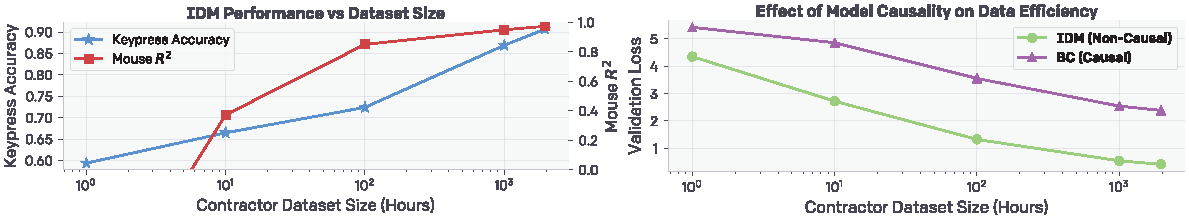
\includegraphics[width=\linewidth]{assets/First_IDM_Results.pdf}
\end{center}
\vspace{-8px}
\caption{\textbf{(Left)} IDM keypress accuracy and mouse movement $R^2$ (explained variance\cite{steel1960principles}) as a function of dataset size. \textbf{(Right)} IDM vs.\ behavioral cloning data efficiency.}
\label{fig:first_idm_results}
\end{figure}

The IDM architecture is comprised primarily of a temporal convolution layer, a ResNet\cite{he2016deep} image processing stack, and residual unmasked attention layers, from which the IDM simultaneously predicts keypresses and mouse movements (see Appendix \ref{appendix:training_details_IDM} for IDM architecture and training details).
A key hypothesis behind our work is that IDMs can be trained with a relatively small amount of labeled data.
While more data improves both mouse movement and keypress predictions, our best IDM trains on only 1962 hours of data (compared to the $\sim$70k hours of clean data we collected from the internet) and achieves 90.6\% keypress accuracy and a 0.97 $R^2$ for mouse movements evaluated on a held-out validation set of contractor-labeled data (Figure \ref{fig:first_idm_results} left).

Figure~\ref{fig:first_idm_results} (right) validates our hypothesis that IDMs are far more data efficient than BC models, likely because inverting environment mechanics is far easier than modeling the entire distribution of human behavior. The IDM is two orders of magnitude more data efficient than a BC model trained on the same data and improves more quickly with more data.
This evidence supports the hypothesis that it is more effective to use contractor data within the VPT pipeline by training an IDM than it is to train a foundation model from contractor data directly (Sections \ref{section:foundation_data_scaling} and \ref{section:idm_data_scaling} provide additional evidence).